%% LaTeX2e class for student theses
%% sections/evaluation.tex
%% 
%% Karlsruhe Institute of Technology
%% Institute for Program Structures and Data Organization
%% Chair for Software Design and Quality (SDQ)
%%
%% Dr.-Ing. Erik Burger
%% burger@kit.edu
%%
%% Version 1.3.2, 2017-08-01

\chapter{Evaluation}
\label{ch:eval}
In this chapter, we evaluate the process to create a case on the basis of the application to the CoCoME system. Also, the created case study is evaluated. Then PCM modeling language is evaluated, if it is possible to express the created case study. At last, the results of the evaluation are discussed to conclude this chapter.
\section{GQM plan}
Three aspects of the thesis are evaluated. First, the applicability of the introduced method, secondly the usability of the created case study for data based privacy analysis and and last but not least to what extent it is possible to model the created case study with PCM. 
%Reicht das als Hinweis ?
 Each evaluation follow a GQM plan \cite{GQM_Intro}, which is shown in \autoref{GQMPlan}. 
\begin{figure}
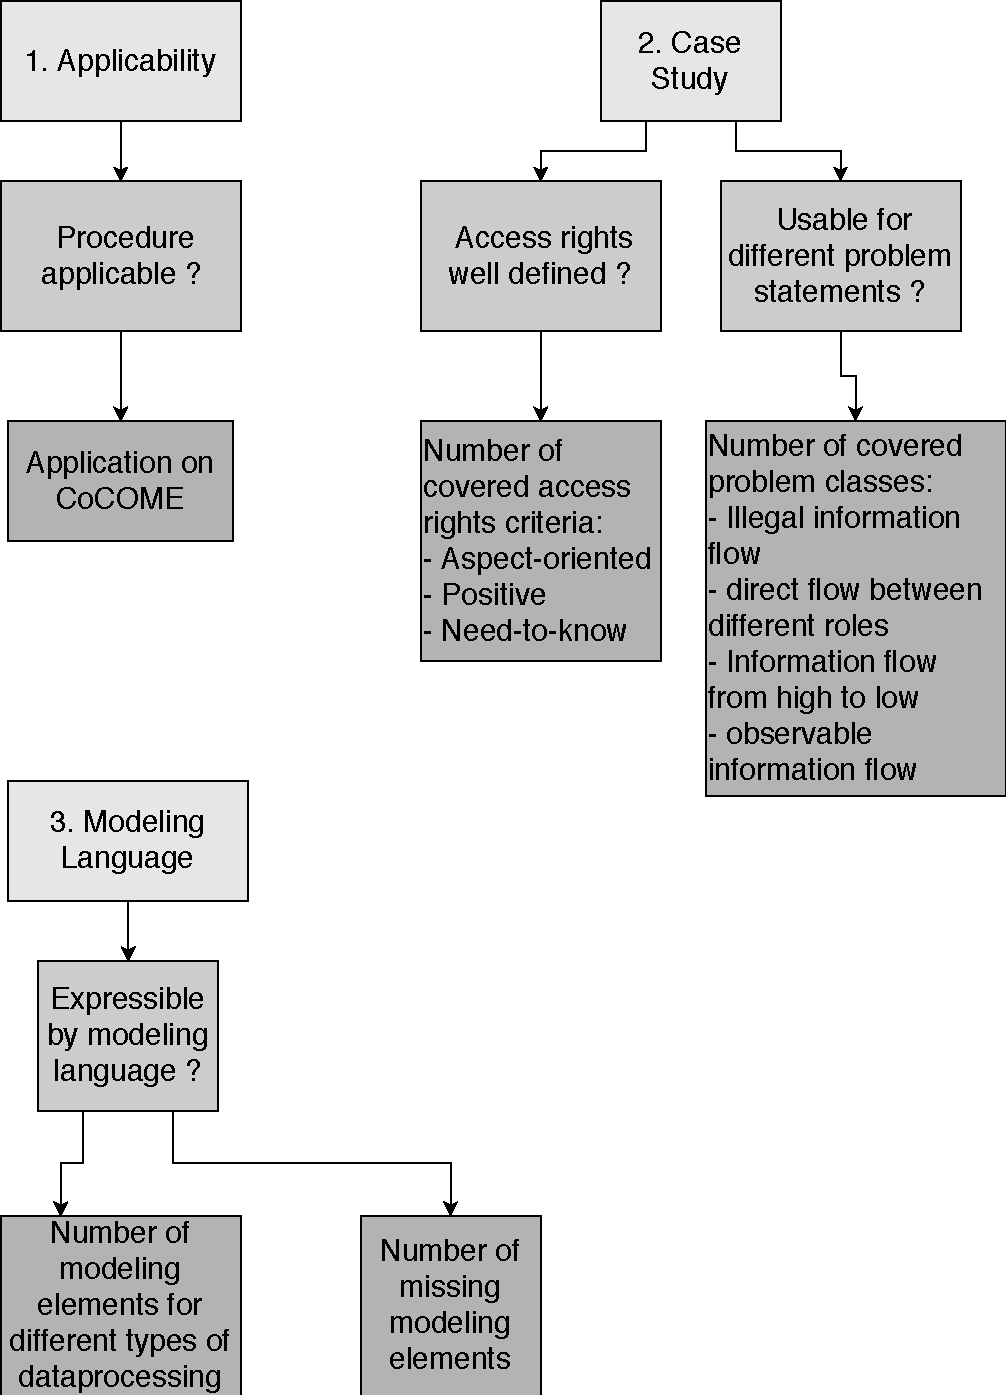
\includegraphics[scale=.8, origin=c ]{logos/OverviewEval.pdf}
\caption{The GQM plan for the three parts of the evaluation. Each part is divided into }
\label{GQMPlan}
\end{figure}
\section{Applicability of the introduced method}
The first aspect we want to evaluate is applicability of the introduced method for software systems. We check this so the method an be used to create further case studies. 
\subsection{Is the introduced method applicable to a concrete system}
To verify if the goal is achieved, we defined the following question:\\
Is the method applicable for a system that models a PickupShop?\\
Pickupshop in this case means, that orders are placed online and picked up later by the customer.
As a metric for answering the question, we take the successful application of the method to CoCoME. 
\subsubsection{Application to the CoCoME system}
In the chapters \autoref{ch:cocome} and \autoref{casestudysystem}, the application of the method to CoCoME is shown. It is possible to create case study for the CoCoME. We followed the steps described in chapter \nameref{ch:method} and after all the steps were taken we successfully created a case study. The use to carry out data-based data protection analyses is evaluated in  \autoref{usage_DBPA}. In \autoref{casestudysystem} we successfully created a case study for the examined excerpt. Therefore, we concluded that the method is applicable for the reduced system.
\section{Usability of the created case study for data-based privacy analysis}
\label{usage_DBPA}
The next aspect we evaluated the usability of the created case study. A case study is not useful if it does not meet criteria. The criteria ensure that the case study is in a state where it can be used for data-based data privacy analysis. To ensure this, we evaluate two different parts of the case study. First, we evaluate the defined access rights, then the defined data flows. 
\subsection{Are the access rights well defined ?}
Well defined access rights means in this context that the defined access rights meet the criteria defined by Evered and Bögeholz\cite{CaseStudyAndAccessrigths}.The two authors defined seven different criteria. In order to ensure clearly defined access rights, the defined criteria should be met. In our case, it is not possible to evaluate all seven criteria. This seven criteria are : Concise, clear, aspect-oriented, fundamental, positive, need-to-know and efficient. Clear and concise are omitted, because for the verification of these two criteria a survey is needed. It was also not possible to check the fundamental criterion, because it needs code to verify if the access rights are embedded in it. At last the efficient criterion also needs running code. This criterion measures the overhead that access rights cause in a system. Since the thesis is oriented on the conceptual level instead of on a code level, this criterion was not included in our scope. 
%Gewählte Kriterien beschreiben
The three chosen criteria that we are utilizing for our evaluation are aspect-oriented, positive and need to know. The criterion aspect-oriented describes that the access rights should be separated from the code. This allows a better understanding of the code and more importantly it allows that different code is used in different contexts. The criterion positive describes, that each access to data classes must be explicitly given to a subject. The default value for access rights is no access. The criterion need-to-know describes the state of access rights where each role has just access to the absolute necessary data that is used to fulfill the tasks of the role.This criterion intends to ensure that access rights are define fine-grained. To give a simple example, a role requires the customer address to perform its tasks.  Fine-grained access rights ensure that the role can only access the address data. Access to other customer data must then be restricted.\\ The number of met criteria is the metric to answer the question. The evaluation of the access rights has to be taken with a grain of salt. Since the access rights are dependent on the security relevant data, the defined roles and the system model, the access rights needs to be reviewed each time one of the dependencies changes.
\subsubsection{Number of satisfied criteria}
The evaluation is done in a checklist manner. For each criterion the defined access rights are evaluated whether they fulfill this criterion. 
\paragraph{Aspect-oriented}
%Beschreibung des Kriteriums danach 
The access rights are stored separately from the code and even from the data flows. The access rights are changeable in the context of the case study. This allows that a scenario may be evaluated in different security contexts. So this criterion is met
\paragraph{Positive}
The created case study achieves this criterion. First, granular access control rights have been defined. The access rights are differentiated in four different levels. We also defined a default value, which represents \textit{no access} to data.
\paragraph{Need-to-know}
This criterion is achieved by the created case study. We split the data in four classes. For each component it is defined which role has access to which data. With this we can model, for example, that the support employee may access customer data in the Tradingsystem:inventory, but not in Tradingsystem:cashdeskline. The role doesn't need access to customer data in Tradingsystem:cashdeskline for its tasks. It is possible to model that each role only get access to the absolutely necessary data in a component. So this criteria is met.
\subsection{Is the created case Study usable for different information flow classes?}
To verify if a case study system is created that may be used to for data-based privacy analysis, we evaluated as a second aspect, the defined data flows. The following question is defined to indicate whether the goal is reached:\\
Is the created case study usable for different problem statements?\\
In the evaluation we only check the problem statement \textit{Non-influence} \cite{Noninfluence}. Non-influence combines two sub problem statements, \textit{Non-interference} and \textit{Non-leakage}. Non-inference describes that no role may acquire informations from a role that inherits a higher security level. Non-leakage describes the issue that it is not observable what specific actions are performed by a system. All in all the problem statements comes down to different classes of information flow. So we use the different information flow classes as a metric to verify the question. This is done in a checklist manner. 
\subsubsection{Number of different covered information flow classes}
We evaluate the variety of covered information flow classes for the defined scenarios int the case study. We defined four information flow classes to cover non-interference and non-leakage. The covered information flow classes are: Illegal information flow, information flow from higher security levels to lower ones, observable information flow and direct informations flow between roles.  
\begin{itemize}
\item Illegal information flow \\
This class includes the information flow of data to roles that  have no access to data of this type. %TODO nochmal genau reingehen
\item Information flow from higher security levels to lower ones\\ In the thesis, we use data flows as the main source of informations. The data is altered with specific operations. So our definition for information flow from high to low is: a sequence of actions, so that is possible for a role that inherit a certain security level to get access to data that are only accessible by higher security levels. 
\item Observable information flow \\ This class describes if the data flow are observable from the outside and to determine, for example, if a security relevant operation is performed. The acquired informations may be used for an attack on the system.
\item Direct information flow between roles\\ This information flow class models data flow between two roles while both interact simultaneously with a system. This refers especially to the security relevant data that may be transferred between two roles with different security levels.
\end{itemize}
\paragraph{Illegal information flow}
The first scenario model illegal data flow. The stock manager in this scenario has access to the ID of an customer. the role has no rights to have access customer related data. Then, the stock manager request a report of this specific customer and receives a full report for this customer. The stock manager has the security level \textit{AccessToUSedData}. The report for one customer is no necessary data for the stock manager to perform its tasks. In this scenario an illegal data flow is modeled. Therefore, the illegal data flow class is part of the created case study.
\paragraph{Information flow from higher security levels to lower ones}
For each data type in each component the access for each role is regulated, therefore it is possible that the security levels change. To check if the information flow is in place, we have analyzed the data flows to determine if a role within the data flow is accessing  unauthorized data.  
\paragraph{Observable information flow}
We did not change the base system of CoCoME. In the base system of CoCoME it is possible to observe when, for example, users finish authenticating, because they are then allowed to perform different actions. So this information flow class is not modeled in a scenario. 
\paragraph{Direct information flow between roles} For the fact that no scenario with more than one role is defined, this class is also not covered in the case study.
\section{Expressiveness of data centric PCM}
The last evaluation aspect of this thesis is to evaluate the chosen modeling language, in this case data-centric PCM. We want to check to what extent PCM is able to add the access rights and data flows in the already existing system model. To allow the extension, Seifermann \cite{MMextension} provided a meta model extension. This meta model extension is the central point of the evaluation. Without the meta model extension, PCM is not able to store data flows and access control rights directly in a system model. 
\subsection{Is the created case study expressible with PCM ?}
A as metric to verify if the, we use the created case study and check if all operations for the different types of data are expressible by PCM. Also we check if elements for types of data processing are missing. The metric is done in a checklist manner. 
\subsubsection{Number of available elements to model the different types of data processing}
First we measure in what current state the operations of the meta model extension are in. We identified five types of data processing that are needed to express the data flows. Currently twelve operations are available in the meta model extension. We measure which operation express the which type of data processing.
\paragraph{Operations relational algebra}
This type of data processing describes the manipulation of database or data requested from databases. The operations for this are available in the meta model. 
\paragraph{I/O- operations}
This type of data processing describes an I/O operation in the data flow, where a user receives data and inputs the same or an other data type in the system. An operation for this is available. 
\paragraph{Transmission data}
This data type describes if component transmit types of data. An operation for this available in the meta model extension. 
\paragraph{Change Access rights}
In the course of a data flow it may happen, that the access right level of a data type changes. For this case an operation in the meta model extension is available. This mostly happens when an operation changes the type of data. This type of processing is closely related to the next one described. 
\paragraph{Alternation of data}
This is a larger type of operations. All in all, this type describes the alternation of data. This includes
creation of data, merging many points in , for example, into list or set. Also the splitting data, like lists, in the different data points. This type of data processing describes the contrasting operation to merging data in collections. 
\subsection{Number of missing elements for the different }
An element for modeling the ACM in the system model is missing.
\section{Discussion}
After all the evaluations are conducted, we discuss the findings. This discussion will be divided into three parts. Each parts covers one of the evaluation aspects shown in \autoref{GQMPlan}.\\
We were able to verify that the method is applicable to a system that models a pickup shop. The method should also be applied to other systems. Possible other systems are flight booking systems, food suppliers, etc. The weakness in this part of the evaluation is that the method has not been applied often enough to different systems to make a statement about its applicability.\\
In the next part, the evaluation results of the access rights and data flows are discussed. First, the defined access rights in the case study. We evaluated based on predefined criteria by Evered and Bögeholz \cite{CaseStudyAndAccessrigths} the access rights. Not all criteria were applicable to the case study, because for some criteria one need running code which is not in the scope of the case study. Other criteria weren't applicable due to time constraints. All in all, as shown in \autoref{eval_AR}, we achieved with our definition of the access rights all three criteria. There is surely some work to be done to allow to check more criteria, like conducting a survey for the criteria clear and concise. For the criteria fundamental and efficient a deployment of CoCoME which includes the access rights is needed. The evaluation of the access rights has to be taken with a grain of salt. Since the access rights depend on the security-relevant data and the roles defined in the system, they must be reevaluated if something has changed.  The evaluation is therefore only a snapshot of the current quality of the access rights. Next, we discuss the evaluation for the different covered information flow classes. We achieved to cover two of the four information flow classes, which is a pretty solid. As we see it, the desirable state is to cover all information flow classes in width and depth. Width means that at least each class is covered by at least one data flow. Depth means that for each class a data flow is defined that is illegal for the class and one that it is not.As shown in \autoref{eval_DF}, we only cover two information flow classes. 
At last we discuss the results for our modeling language PCM. We defined five types of data processing and evaluated whether they are possible to model in PCM. The result is shown in \autoref{eval_MM}. As shown, all types of data processing are modeled. Therefore, we conclude it is be possible to model all created case studies with PCM. But it is not possible to store the ACM in the same model. 
\begin{table}
\begin{tabular}{|c|c|}
\hline 
Access Rights & fulfilled ? \\ 
\hline 
Aspect-oriented & yes \\ 
\hline 
Positive & yes \\ 
\hline 
Need-to-know & yes \\ 
\hline 
\end{tabular} 
\caption{Overview of the evaluation result for the access rights.}
\label{eval_AR}
\end{table}

\begin{table}
\begin{tabular}{|c|c|}
\hline 
Data flow & fulfilled \\ 
\hline 
Illegal information flow & yes \\ 
\hline 
Information flow from high to low & yes \\ 
\hline 
Observable information  flow & no \\ 
\hline 
Direct information flow between roles & no \\ 
\hline 
\end{tabular} 
\caption{Overview over the evaluation result for the data flows.}
\label{eval_DF}
\end{table}
 
\begin{table}
\begin{tabular}{|c|c|}
\hline 
Meta model  & possible ? \\ 
\hline 
relational algebra & yes \\ 
\hline 
I/O operations & yes \\ 
\hline 
Transmission of data & yes \\ 
\hline 
Change of access rights & yes \\ 
\hline 
Alternation of data & yes \\ 
\hline 
ACM in system model & no \\
\hline
\end{tabular} 
\caption{Overview over the results for the evaluation of PCM.}
\label{eval_MM}
\end{table}
To conclude the evaluation, one can say that we introduced an applicable method for a certain typ eof systems to create data flows for a data-based privacy analysis. For the sample case study, we say it is a proof-of-concept, because only two class of information are modeled. The defined access rights are well defined in the current evaluation, but it is imperative to apply the other criteria to get a more complete picture. It must also be said that access rights are relatively volatile, as there is a need to check even small changes in the system. At last, the used modeling language is able to model all types of data processing and is therefore usable for data-based privacy analysis. The only throwback for the modeling language is that the ACM must be stored separately, this may lead to inconsistency and should be fixed soon.
